\chapter{Execução à nível de Programa}

  Esse capítulo apresenta as atividades e resultados obtidos na execução do processo a nível de Programa.
  
  \begin{figure}[!htbp]
    \centering
    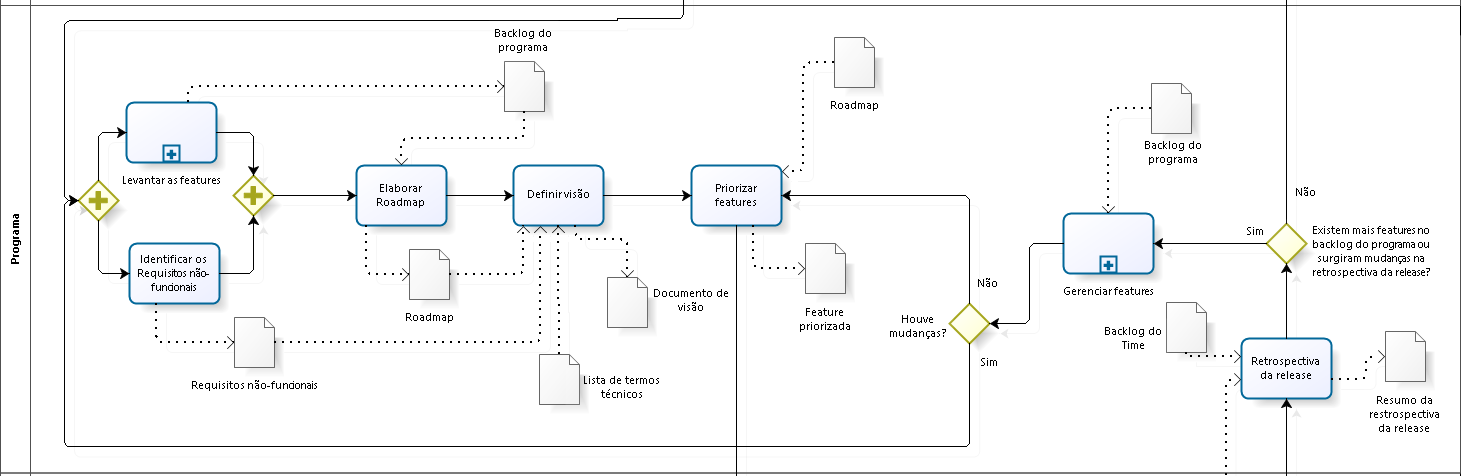
\includegraphics[scale=0.33]{figuras/processo_programa}
    \caption[Processo - Nível de Programa]{Processo - Nível de Programa.}
    \label{processo_programa}
  \end{figure}
  \vspace{0in}
  
  \section{Reuniões realizadas}
    
    A nível de programa foram realizadas duas reuniões com o cliente, que são brevemente resumidas nesta seção.
    
    \subsection{Resumo da 1ª reunião}
    
      No contexto do nível de Programa, a primeira reunião realizada utilizou a técnica de \textit{workshop}
      com \textit{brainstorming} para o levantamento das \textit{features} e dos requisitos não-funcionais da aplicação.
      A equipe de requisitos planejou o \textit{workshop} segundo a agenda apresentada na figura \ref{agenda_workshop}.
      
      \begin{figure}[!htbp]
	\centering
	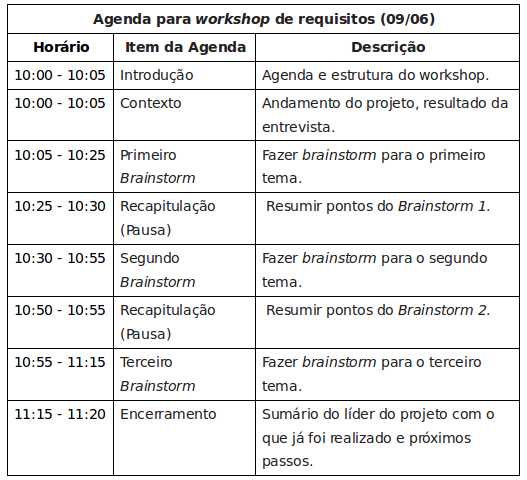
\includegraphics[scale=0.5]{figuras/agenda_workshop}
	\caption[\textit{Agenda do \textit{workshop} de requisitos} do projeto]{Agenda do \textit{workshop} de requisitos.}
	\label{agenda_workshop}
      \end{figure}
      
      Os temas dos \textit{brainstorms} eram, respectivamente, atividades da gestão operacional, atividades da gestão administrativa
      e questões referentes ao funcionamento e comportamento do sistema (requisitos não-funcionais). As ideias e colocações 
      geradas nos \textit{brainstorms} foram registradas em \textit{Post-its} pelos participantes do \textit{brainstorm}. 
      A figura \ref{post_its_reuniao} ilustra os resultados dos \textit{brainstorms} realizados.
      
      \begin{figure}[!htbp]
	\centering
	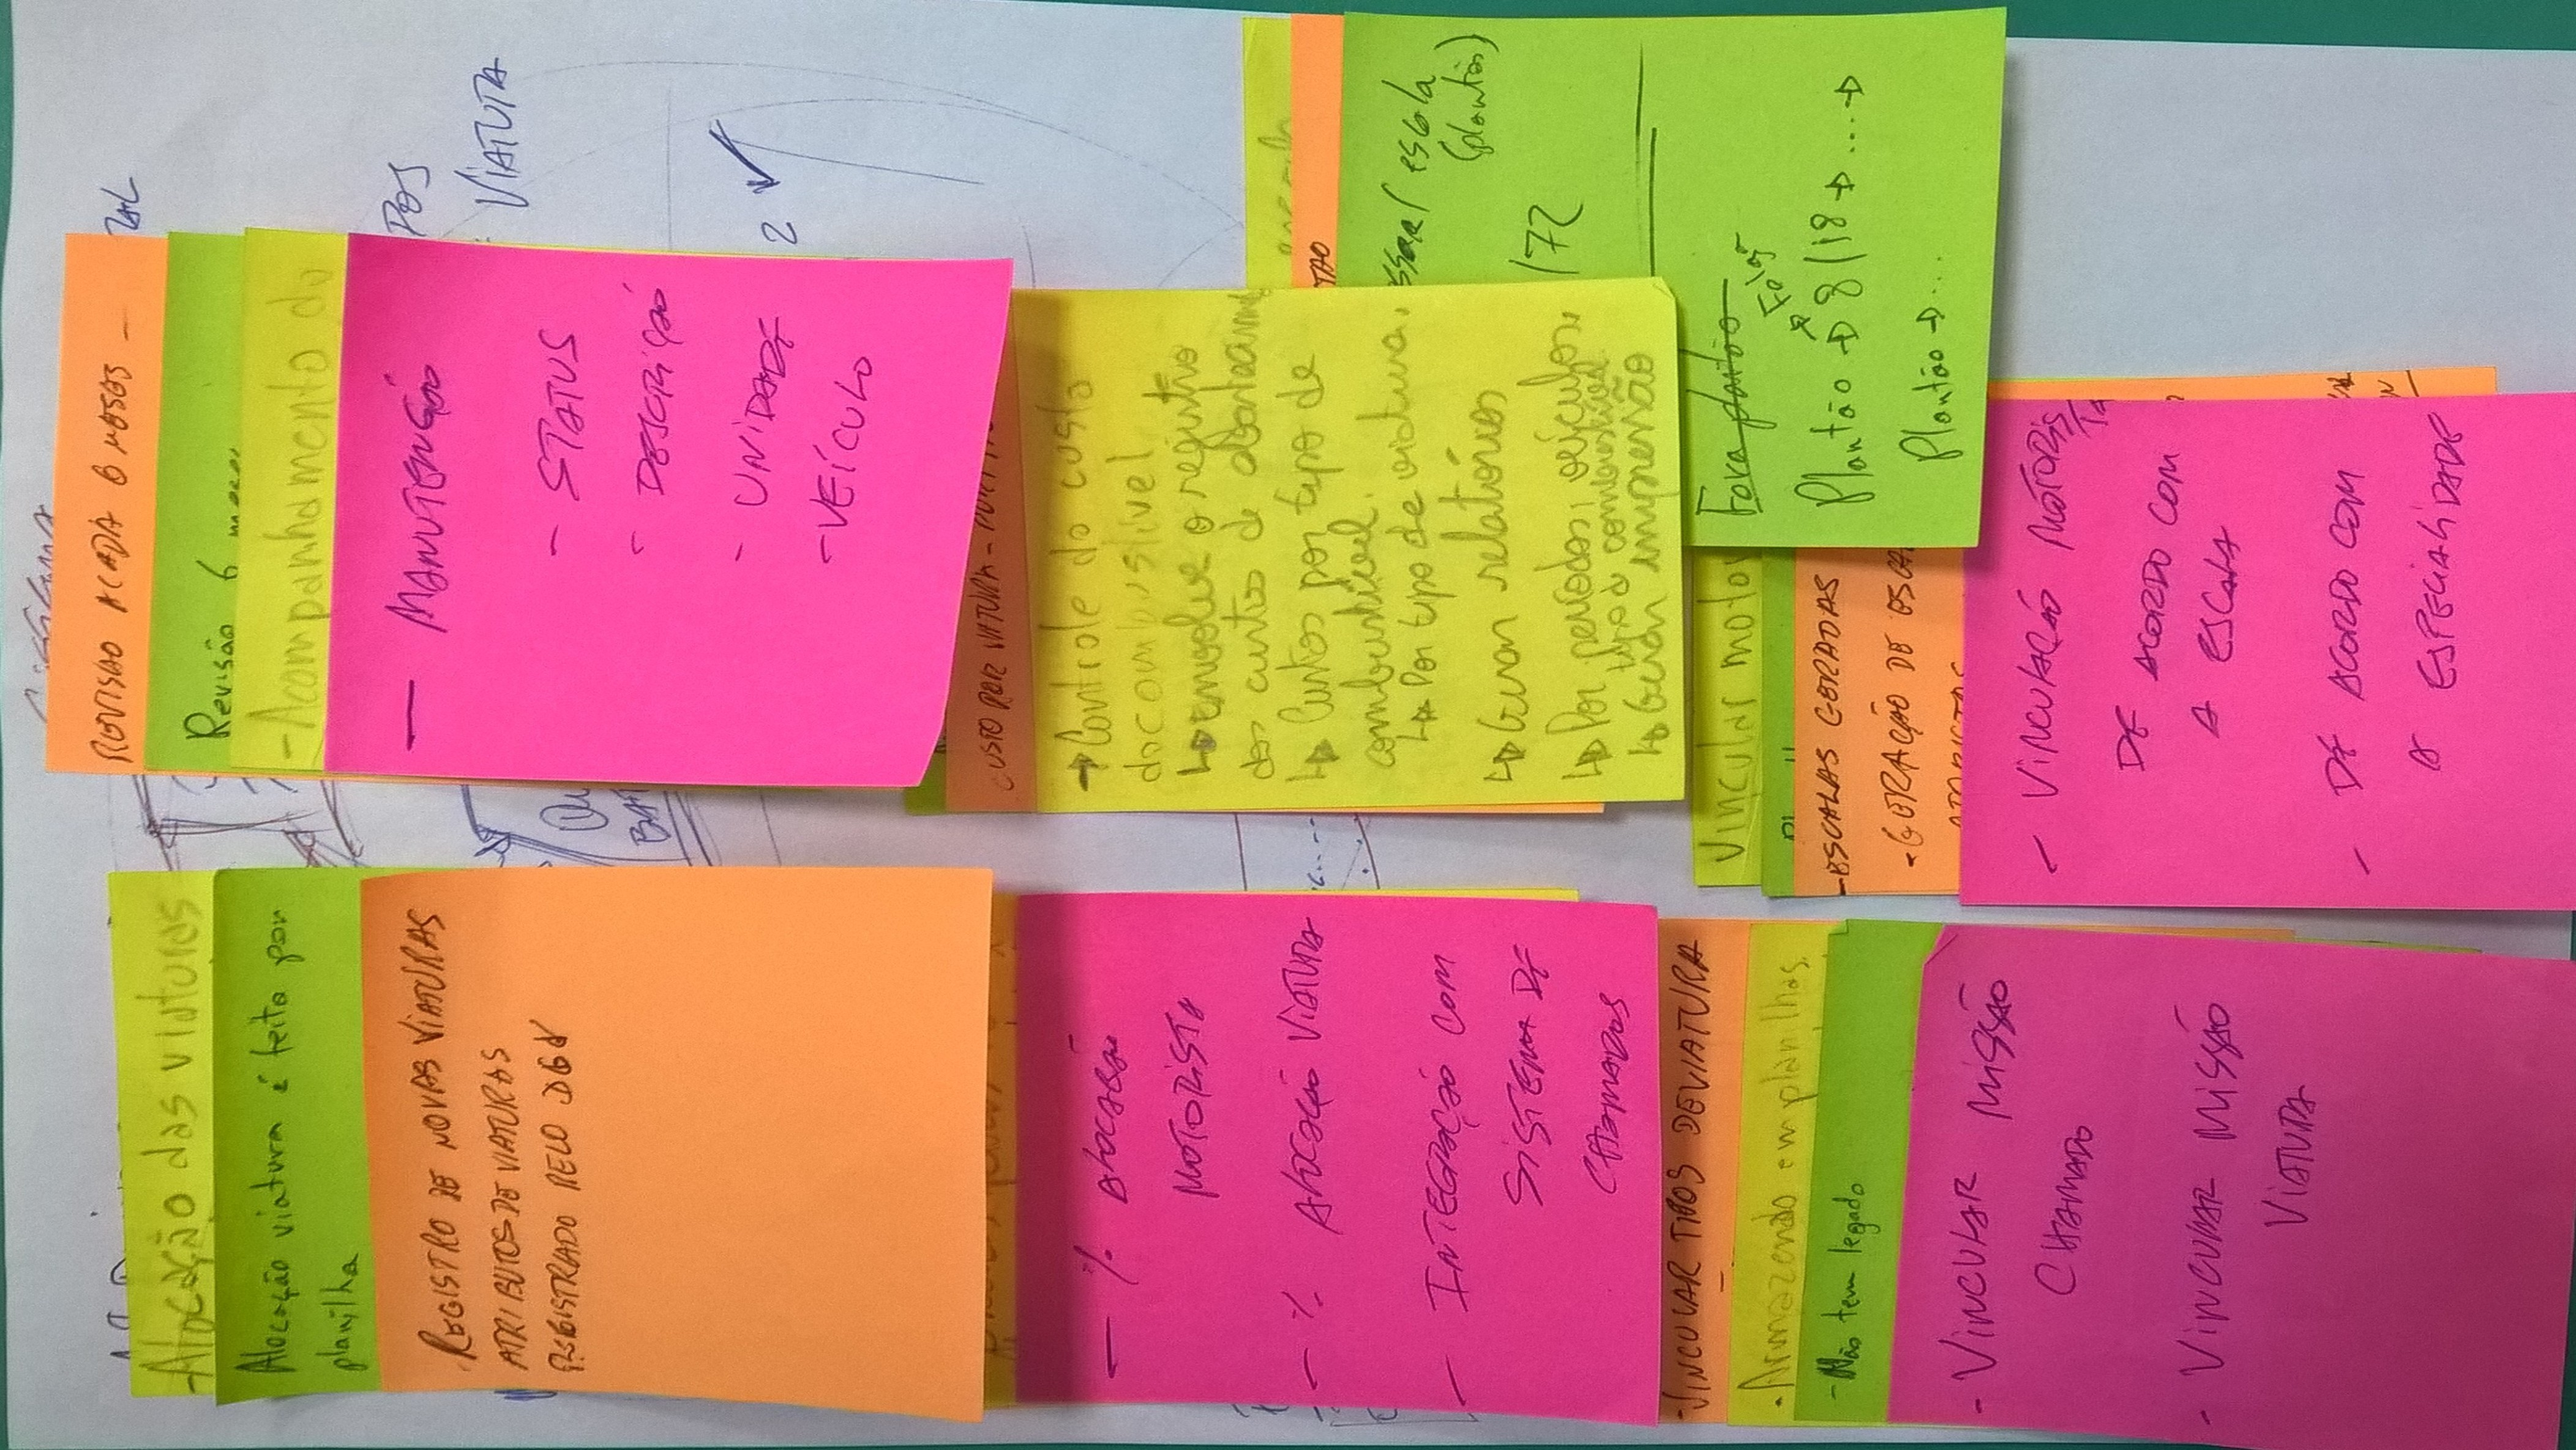
\includegraphics[scale=0.11]{figuras/post_its_reuniao}
	\caption[\textit{Post-its} com as colocações feitas no \textit{brainstorm}]
	  {\textit{Post-its} com as colocações feitas no \textit{brainstorm}.}
	\label{post_its_reuniao}
      \end{figure}
      
      Na prática, a reunião começou a nível de Portfólio quando foi validado com o cliente a priorização dos épicos
      (atividade de Priorizar épicos a nível de Portfólio). A partir dos épicos priorizados (segundo o cliente, os épicos tinham a 
      mesma relevância), conceitualmente, a reunião desceu para o nível de Programa com a realização dos \textit{brainstorms},
      realizando as atividades de "Levantar as \textit{features}" e "Identificar os requisitos não-funcionais" do nível de programa.
      
      Com os pontos discutidos nessa reunião, ainda foi possível levantar alguns requisitos funcionais do sistema.
  
  \section{Considerações finais a nível de Programa}
    
    Esta seção apresenta um resumo dos itens mais importantes produzidos a nível de Portfólio.
    
    \subsection{\textit{Features} identificadas}
      
      O \textit{Backlog} do Programa ficou composto pelas seguintes \textit{features}:
      
      \begin{itemize}
       \item \textit{Feature} 1 (E1F1) - Gerenciamento das missões de unidade;
       \item \textit{Feature} 2 (E1F2) - Gerenciamento dos dados dos abastecimentos das viaturas;
       \item \textit{Feature} 3 (E1F3) - Consulta das viaturas das unidades por dispositivo móvel. 
       \item \textit{Feature} 4 (E2F1) - Gerenciamento dos motoristas da unidade;
       \item \textit{Feature} 5 (E2F2) - Gerenciamento das viaturas da unidade;
      \end{itemize}
      
      As \textit{features} estão descritas mais detalhadamente no documento de visão (apêndice \ref{doc_visao}).
    
    \subsection{Requisitos Não-funcionais}
      
      
      
    \subsection{\textit{Roadmap}}
      
      
    \subsection{Visão}
    
      